%!TEX root = foglio.tex

\subsection{Trasformazione var continua:}

Sia $X:\Omega \rightarrow \mathbb{R}$ va continua con densità $f_{X}$ e $Y=g(X)$, con $g$ monotona e $g^{-1}=h \in \Cc^{1}$. Allora $X=h(Y)$ e dunque $f_{Y}(y)=f_{X}\left(h(y)\right)\left|\frac{\de}{\de y} h(y)\right|$

\subsection{Delta di Dirac:}

$\delta_{n}$ è tc $\PP(X=n)=1$

\subsection{Continua uniforme:} 

$\Uc(a, b)$

$f(x)=\frac{1}{b-a} \Ind_{[a,b]}(x), F(x)=\frac{x-a}{b-a}$

$\mathbb{E}[X]=\frac{a+b}{2}\quad \operatorname{Var}(X)=\frac{(b-a)^{2}}{12}$

$1-\Uc(0,1)\sim\Uc(0,1)$

\subsection{Bernoulli:} 

$\operatorname{Be}(p)$

$f(x)=p^x(1-p)^{1-x}\Ind_{\{0,1\}}(x)$

$\mathbb{E}[X]=p\quad \operatorname{Var}(X)=p(1-p)$

$\sum \Be(p)=\Bi(n,p)$

$1-\Be(p)\sim\Be(1-p)$

\subsection{Binomiale:} 

$\Bi(n, p)$

$\PP(X=x)=\binom{n}{x}p^x(1-p)^{n-x}$

$\mathbb{E}[X]=n p\quad \operatorname{Var}(X)=n p(1-p)$

$\Bi(n,p)+\Bi(m,p)\sim\Bi(n+m,p)$

\subsection{Geometrica:} 

$\mathcal{G}(p)$ è il numero di fallimenti prima di un successo in un processo di Bernoulli. Priva di memoria.

$\PP(X=k)=p(1-p)^{k-1}$

$F(k)=\PP(X \leq k)=1-\PP(X \geq k+1)=1-(1-p)^{k}$

$\mathbb{E}[X]=\frac{1}{p} \quad \operatorname{Var}(X)=\frac{1-p}{p^{2}}$

\subsection{Geometrica traslata:} 

$\PP(W=k)=p(1-p)^{k}$

\subsection{Poisson:}

$\Pc(\lambda)$ legge degli eventi rari. Limite delle distribuzioni binomiali con $\lambda=n p$.

$\PP(X=k)=e^{-\lambda} \frac{\lambda^{k}}{k !}\Ind_\NN \quad \mathbb{E}[X]=\lambda \quad \operatorname{Var}(X)=\lambda$

$\Pc(\lambda)+\Pc(\mu)\sim\Pc(\lambda+\mu)$ (se $\Perp$)

\subsection{Normale:} 

$\mathcal{N}\left(\mu, \sigma^{2}\right)$

$f(x)=\frac{1}{\sqrt{2 \pi \sigma^{2}}} \exp \left\{-\frac{(x-\mu)^{2}}{2 \sigma^{2}}\right\}$

$\mathbb{E}[X]=\mu \quad \operatorname{Var}(X)=\sigma^{2}$

$\mathbb{E}\left[X^{4}\right]=\mu^{4}+6 \mu^{2} \sigma^{2}+3 \sigma^{4} \quad \mathbb{E}\left[(X-\mu)^{4}\right]=3 \sigma^{4}$

$\PP(x \leqslant t)=\PP\left(\frac{X-\mu}{\sigma} \leqslant \frac{t-\mu}{\sigma}\right)=$ \\
$\text{}\quad=\PP\left(Z\leqslant \frac{t-\mu}{\sigma}\right)=\phi\left(\frac{t-\mu}{\sigma}\right)$ con $Z=\frac{X-\mu}{\sigma} \sim \mathcal{N}(0,1)$

$\phi(-z)=1-\phi(z) \quad \mathbb{P}(|Z|>z)=2(1-\phi(z)) \quad \phi(k)<0.1\ \Rightarrow\ k<-z_{1-0.1}$

$\mathcal{N}\left(m, s^{2}\right)+\mathcal{N}\left(n, r^{2}\right)\sim\mathcal{N}\left(m+n, s^{2}+r^{2}\right)(\mathrm{se} \Perp)$

$\Nc(\mu,\sigma^2_{\text{nota}})\ \Rightarrow\ X_1|\sum X_i=t\sim\Nc\left(\frac{t}{n},\frac{n-1}{n}\sigma^2\right)$

\subsection{Lognormale:} 

$\log \mathcal{N}\left(\mu, \sigma^{2}\right)\  X=e^{\mathcal{N}}$

$f(x)=\frac{1}{x \sqrt{2 \pi \sigma^{2}}} \exp \left\{-\frac{(\ln x-\mu)^{2}}{2 \sigma^{2}}\right\} \Ind_{(0,+\infty)}$

$F(x)=\Phi_{(\mu, \sigma)}(\ln x)$

$\mathbb{E}[X]=e^{\mu+\sigma^{2} / 2} \quad \operatorname{Var}(X)=e^{2 \mu+\sigma^{2}}\left(e^{\sigma^{2}}-1\right)$

\subsection{Chi-quadro:} 

$\left(\chi^{2}(k)\right)$

$f(x)=\frac{1}{2^{k / 2} \Gamma(k / 2)} x^{k / 2-1} e^{-x / 2} \Ind_{(0,+\infty)}$

$\mathbb{E}[X]=k \quad \operatorname{Var}(X)=2 k$

$\chi^{2}(n)=\Gamma\left(\frac{n}{2}, \frac{1}{2}\right)$

$\sum Z^2\sim\chi^2(n) \quad \frac{\sum(X_i-\mu)^2}{\sigma^2}\sim\chi^2(n)$

$Z^{2} \sim \Gamma\left(\frac{1}{2}, \frac{1}{2}\right)=\chi^{2}(1)$

\subsection{T di student:}

$t(n)$ costruita come $\frac{Z}{\sqrt{Q/n}}$ con $Z \Perp Q$

$f(x)=\frac{\Gamma\left(\frac{n+1}{2}\right)}{\Gamma\left(\frac{n}{2}\right) \sqrt{\pi n}} \cdot \frac{1}{\left(1+\frac{x^{2}}{n}\right)^{\frac{n+1}{2}}}$

$\mathbb{E}[T]=0$ se $n>1$ oppure indefinito.

$\operatorname{Var}(T)=\frac{n}{n-2}$ se $n>2$ oppure indefinita.

\subsection{Esponenziale:} 

$\mathcal{E}(\lambda)$ è la durata di vita di un fenomeno. Priva di memoria.

$f(x)=\lambda e^{-\lambda x} \Ind_{(0,+\infty)}(x) \quad F(x)=1-e^{-\lambda x}$

$\mathbb{E}[X]=\frac{1}{\lambda}\quad \operatorname{Var}(X)=\frac{1}{\lambda^{2}}$

$a\Ec(\lambda)\sim\Ec\left(\frac{\lambda}{a}\right)$

$X_{i} \sim \mathcal{E}(\lambda)\ \Rightarrow\ X_{(1)} \sim \mathcal{E}(n \lambda)$

$X_i\sim\Ec(\theta)\ \Rightarrow\ \sum X_i\sim\Gamma(n,\theta)\ \Rightarrow\ \Xn\sim\Gamma(n,n\theta)$

$Y\sim f_Y=e^{\theta-y}\Ind_{(\theta,+\infty)}\ \Rightarrow\ Y\sim\theta+\Ec(1)$ \\
$\text{}\quad\Rightarrow\ Y_{(1)}\sim\theta+\Ec(n)\ \Rightarrow\ f_{Y_{(1)}}=ne^{-n(y-\theta)}\Ind_{(\theta,+\infty)}$

$Y\sim f_Y=\frac{1}{\theta}e^{-\frac{x-\theta}{\theta}}\Ind_{(\theta,+\infty)}\ \Rightarrow\ Y\sim\theta+\Ec\left(\frac{1}{\theta}\right)$

\subsection{Gamma:} 

$\Gamma(\alpha, \lambda)$ è la somma di $\alpha$ esponenziali $\Ec(\lambda)$

$f(x)=\frac{\lambda^{\alpha} x^{\alpha-1} e^{-\lambda x}}{\Gamma(\alpha)} \mathbb{1}_{(0,+\infty)}(x)$

$F(x)=\left(1-\sum_{k=0}^{\alpha-1} e^{-\lambda x} \frac{(\lambda x)^{k}}{k !}\right)=\frac{\gamma(\alpha, \lambda x)}{\Gamma(\alpha)}$

$\mathbb{E}\left[X^{k}\right]=\frac{\alpha(\alpha+1) \ldots(\alpha+k-1)}{\lambda^{k}} \quad \EE[X]=\frac{\alpha}{\lambda}\quad\EE[X^2]=\frac{\alpha(\alpha+1)}{\lambda^2}$

$\EE\left[\frac{1}{\Gamma(n,\theta)}\right]=\frac{\theta}{n-1}\quad \EE\left[\frac{1}{\Gamma(n,\theta)^2}\right]=\frac{\theta^2}{(n-1)(n-2)}$

$\Gamma(\alpha)=\int_{0}^{+\infty} x^{\alpha-1} e^{-x} \dx$

$\Gamma(n+1)=n!\quad \Gamma(n)=(n-1)!$

$\Gamma(1)=1\quad \Gamma\left(\frac{1}{2}\right)=\sqrt{\pi}$

$Y=c X \sim \Gamma\left(\alpha, \frac{\lambda}{c}\right) \operatorname{con} c>0$

$\Gamma(\alpha,\theta)+\Gamma(\beta,\theta)\sim\Gamma(\alpha+\beta)$ (se $\Perp$)

\subsection{Weibull:} 

$W(\lambda, k),\ \lambda>0,\ k>0$

$f(x)=\frac{k}{\lambda^{k}} x^{k-1} e^{-(x / \lambda)^{k}} \Ind_{(0,+\infty)}(x)$

$F(x)=1-e^{-\left(\frac{x}{\lambda}\right)^{k}}\quad \mathbb{E}[X]=\frac{\lambda}{k} \Gamma\left(\frac{1}{k}\right)$,

$\operatorname{Var}(X)=\frac{\lambda^{2}}{k^{2}}\left[2 k \Gamma\left(\frac{2}{k}\right)-\Gamma^{2}\left(\frac{1}{k}\right)\right]$

$Y\sim W(\alpha,\beta)\ \Rightarrow \ Y^\alpha\sim\Ec(\beta)$

\subsection{Beta:}

$\Bc(\alpha, \beta)$ governa la prb $p$, a priori distribuita unif, di un proc di Bernoulli dopo aver osservato $\alpha-1$ successi e $\beta-1$ insuccessi $(\alpha, \beta>0)$

$f(x)=\frac{\Gamma(\alpha+\beta)}{\Gamma(\alpha)\Gamma(\beta)}x^{\alpha-1}(1-x)^{\beta-1}\Ind_{(0,1)}(x)$

$\mathbb{E}[X]=\frac{\alpha}{\alpha+\beta}$, con $B(x, y)=\int_{0}^{1} t^{x-1}(1-t)^{y-1} \mathrm{~d} t$

$\operatorname{Var}(X)=\frac{\alpha \beta}{(\alpha+\beta)^{2}(\alpha+\beta+1)}$

\subsection{Fisher:}

$\frac{\chi^2(n)/n}{\chi^2(m)/m}=\Fc(n,m)$

\subsection{Ipergeometrica:}

$\Hc(n,h,r)$ descrive l'estrazione senza reimmissione di palline da un'urna con $n$ palline totali, di cui $h$ del tipo $X$ e $n-h$ del tipo $Y$. La prob di ottenere $k$ palline del tipo $X$ estraendone $r$ dall'urna è
\begin{equation*}
p_X(k)=\frac{\binom{h}{k} \binom{n-h}{r-k}}{\binom{n}{r}}
\end{equation*}
($k\in [\max\{0,h+r-n\},\min\{r,h\}]$)

$\EE[X]=\frac{rh}{n}\quad\Var(X)=\frac{h(n-h)r(n-r)}{n^2(n-1)}$

\subsection{Relazione tra le convergenze:}

%!TEX root = foglio.tex

\tikzset{every picture/.style={line width=0.75pt}} %set default line width to 0.75pt        

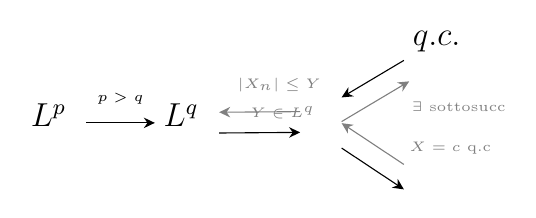
\begin{tikzpicture}[x=0.75pt,y=0.75pt,yscale=-1,xscale=1]
%uncomment if require: \path (0,119); %set diagram left start at 0, and has height of 119

% Text Node
\draw (14,50.4) node [anchor=north west][inner sep=0.75pt]  [font=\large]  {$L^{p}$};
% Text Node
\draw (78,50.4) node [anchor=north west][inner sep=0.75pt]  [font=\large]  {$L^{q}$};
% Text Node
\draw (148,50.9) node [anchor=north west][inner sep=0.75pt]  [font=\large]  {$\PP$};
% Text Node
\draw (198,85.4) node [anchor=north west][inner sep=0.75pt]  [font=\large]  {$\Lc$};
% Text Node
\draw (198,15.4) node [anchor=north west][inner sep=0.75pt]  [font=\large]  {$\text{q.c.}$};
% Text Node
\draw (46,45.4) node [anchor=north west][inner sep=0.75pt]  [font=\tiny]  {$p>q$};
% Text Node
\draw (107,32.9) node [anchor=north west][inner sep=0.75pt]  [font=\tiny,color={rgb, 255:red, 128; green, 128; blue, 128 }  ,opacity=1 ]  {$ \begin{array}{l}
| X_{n}| \leq Y\\
\ \ Y\in L^{q}
\end{array}$};
% Text Node
\draw (197.5,49.5) node [anchor=north west][inner sep=0.75pt]  [font=\tiny,color={rgb, 255:red, 128; green, 128; blue, 128 }  ,opacity=1 ] [align=left] {$\exists $ sottosucc};
% Text Node
\draw (196.5,69) node [anchor=north west][inner sep=0.75pt]  [font=\tiny,color={rgb, 255:red, 128; green, 128; blue, 128 }  ,opacity=1 ] [align=left] {$X=c$ q.c};
% Connection
\draw    (42,61) -- (72,61) ;
\draw [shift={(75,61)}, rotate = 180] [fill={rgb, 255:red, 0; green, 0; blue, 0 }  ][line width=0.08]  [draw opacity=0] (5.36,-2.57) -- (0,0) -- (5.36,2.57) -- (3.56,0) -- cycle    ;
% Connection
\draw [color={rgb, 255:red, 128; green, 128; blue, 128 }  ,draw opacity=1 ]   (109,55.86) -- (145,55.58) ;
\draw [shift={(106,55.88)}, rotate = 359.56] [fill={rgb, 255:red, 128; green, 128; blue, 128 }  ,fill opacity=1 ][line width=0.08]  [draw opacity=0] (5.36,-2.57) -- (0,0) -- (5.36,2.57) -- (3.56,0) -- cycle    ;
% Connection
\draw [color={rgb, 255:red, 0; green, 0; blue, 0 }  ,draw opacity=1 ]   (142,65.6) -- (106,65.88) ;
\draw [shift={(145,65.58)}, rotate = 179.56] [fill={rgb, 255:red, 0; green, 0; blue, 0 }  ,fill opacity=1 ][line width=0.08]  [draw opacity=0] (5.36,-2.57) -- (0,0) -- (5.36,2.57) -- (3.56,0) -- cycle    ;
% Connection
\draw    (167.58,47.2) -- (195,30.89) ;
\draw [shift={(165,48.73)}, rotate = 329.25] [fill={rgb, 255:red, 0; green, 0; blue, 0 }  ][line width=0.08]  [draw opacity=0] (5.36,-2.57) -- (0,0) -- (5.36,2.57) -- (3.56,0) -- cycle    ;
% Connection
\draw [color={rgb, 255:red, 128; green, 128; blue, 128 }  ,draw opacity=1 ]   (194.98,42.53) -- (165,60.37) ;
\draw [shift={(197.56,41)}, rotate = 149.25] [fill={rgb, 255:red, 128; green, 128; blue, 128 }  ,fill opacity=1 ][line width=0.08]  [draw opacity=0] (5.36,-2.57) -- (0,0) -- (5.36,2.57) -- (3.56,0) -- cycle    ;
% Connection
\draw [color={rgb, 255:red, 128; green, 128; blue, 128 }  ,draw opacity=1 ]   (167.5,62.79) -- (195,81.04) ;
\draw [shift={(165,61.13)}, rotate = 33.56] [fill={rgb, 255:red, 128; green, 128; blue, 128 }  ,fill opacity=1 ][line width=0.08]  [draw opacity=0] (5.36,-2.57) -- (0,0) -- (5.36,2.57) -- (3.56,0) -- cycle    ;
% Connection
\draw    (192.5,91.38) -- (165,73.13) ;
\draw [shift={(195,93.04)}, rotate = 213.56] [fill={rgb, 255:red, 0; green, 0; blue, 0 }  ][line width=0.08]  [draw opacity=0] (5.36,-2.57) -- (0,0) -- (5.36,2.57) -- (3.56,0) -- cycle    ;

\end{tikzpicture}

\subsection{Negli spazi} $L^{p}: X_{n} \stackrel{L^{p}}{\longrightarrow} X$ se

$X_{n} \in L^{p} \forall n,\ X \in L^{p}$ e $\mathbb{E}\left[\left|X_{n}-X\right|^{p}\right] \rightarrow 0$

Dato $p \geqslant q \geqslant 1$, conv. in $L^{p} \Longrightarrow$ conv. in $L^{q}$.

Convergono i momenti:

$\mathbb{E}\left[\left|X_{n}\right|^{p}\right] \stackrel{L^{p}}{\longrightarrow} \mathbb{E}\left[|X|^{p}\right]$

Per $p=1$ e $p=2$:

$\mathbb{E}\left[X_{n}\right] \rightarrow \mathbb{E}[X]$ e $\operatorname{Var}\left(X_{n}\right) \rightarrow \operatorname{Var}(X)$

\subsection{Probabilità:} $X_{n} \stackrel{\PP}{\longrightarrow} X$ se

$\forall \varepsilon>0\ \mathbb{P}\left(\left|X_{n}-X\right|>\varepsilon\right) \rightarrow 0$

Esiste una sottosuccessione di $X_{n}$ che converge qc a $X$. Se $X$ appartiene a $L^{p}$ ed è possibile trovare una $Y$ tale che $\left|X_{n}\right| \leqslant Y$ allora questa converge anche in $L^{p}$.

\subsection{Debole:} siano $\mathbb{P}_{n}$ e $\mathbb{P}$ prob su $(\mathbb{R}, \mathcal{B})$. Allora

$\mathbb{P}_{n} \stackrel{\text { deb }}{\longrightarrow} \mathbb{P}$ se $\int_{\mathbb{R}} h\, \de\mathbb{P}_{n} \rightarrow \int_{\mathbb{R}} h\, \de \mathbb{P} \forall h$ cont. e lim.

\subsection{In legge o distribuzione:}

$\text{}$ \\

$X_{n} \stackrel{\Lc}{\longrightarrow} X$ se

$P^{X_{n}} \stackrel{\text { deb }}{\longrightarrow} P^{X}$

Slutsky: $X_{n} \stackrel{\Lc}{\longrightarrow} c \Longrightarrow X_{n} \stackrel{\PP}{\longrightarrow} c$

\subsection{Criteri conv. in legge:}

$X_{n} \stackrel{\mathcal{L}}{\longrightarrow} X$ iff $F_{n}(t) \rightarrow F(t) \forall t$ dove $F$ è cont.

Discreto: $\PP\left(X_{n}=t\right) \rightarrow \PP(X=t) \forall t\in S$ iff $_{n} \stackrel{\Lc}{\longrightarrow} X$ dove $S=S_{X} \cup S_{X_{n}}$

Continuo: $f_{n} \stackrel{q o}{\longrightarrow} f \Longrightarrow X_{n} \stackrel{\mathcal{L}}{\longrightarrow} X$

\subsection{TCL:}

se $X_{i}$ iid con $\mathbb{E}\left[X_{i}\right]=\mu$ e $\operatorname{Var}\left(X_{i}\right)=\sigma^{2}$, allora $\frac{\Xn-\mu}{\sqrt{\sigma^{2} / n}} \stackrel{\Lc}{\rightarrow} \Nc(0,1)$ \\
$\text{}\quad\text{ovvero }\Xn \approx \mathcal{N}\left(\mu, \sigma^{2} / n\right)$

\subsection{LGN:}

Dati $X_{n} \in L^{1}$ iid e $\mu \in \mathbb{R}$, allora \\
$\text{}\quad\mathbb{E}\left[X_{n}\right]=\mu \Longleftrightarrow \Xn \stackrel{q c}{\longrightarrow} \mu$ (vale anche in $L^1,\PP$)

\subsection{Alcune proprietà:}

per un campione gaussiano, si ha:

$\frac{(n-1) S^{2}}{\sigma^{2}} \sim \chi^{2}(n-1)$

$\frac{\Xn-\mu}{\sqrt{S^{2} / n}} \sim t(n-1)$

Doppio val atteso: $\mathbb{E}[\mathbb{E}[X \mid Y]]=\mathbb{E}[X]$

Scomp. varianza: $\operatorname{Var}(X)=\mathbb{E}[\operatorname{Var}(X \mid Y)]+\operatorname{Var}(\mathbb{E}[X \mid Y])$.

\subsection{Metodi delta:}

$\text{}$\\

data $Y_{n}$ t.c $\sqrt{n}\left(Y_{n}-\vartheta\right) \stackrel{\mathcal{L}}{\rightarrow} N\left(0, \sigma^{2}\right)$

$g^{\prime}(\vartheta) \neq 0 \Longrightarrow \sqrt{n}\left(g\left(Y_{n}\right)-g(\vartheta)\right) \stackrel{\mathcal{L}}{\longrightarrow} N\left(0, \sigma^{2} g^{\prime}(\vartheta)^{2}\right)$

$g^{\prime}(\vartheta)=0$ e $g^{\prime \prime}(\vartheta) \neq 0 \Longrightarrow n\left(g\left(Y_{n}\right)-g(\vartheta)\right) \stackrel{\mathcal{L}}{\longrightarrow} \sigma^{2} \frac{g^{\prime \prime}(\vartheta)}{2} \chi^{2}(1)$

\subsection{Funzione generatrice dei momenti}

$$
{\renewcommand*{\arraystretch}{1.8}
\begin{array}{ll}
\text{discreto:} &g(t)=\EE[e^{tX}]=\displaystyle\sum_{i=1}^n p_i e^{tX_i} \\
\text{continuo:} &g(t)=\EE[e^{tX}]=\displaystyle\int_{\RR} e^{tx}f_X(x)\dx \\
\text{gaussiano:} &g(t)=\displaystyle\exp\left\{\mu t+\frac{\sigma^2t^2}{2}\right\}
\end{array}}
$$

Valuto in $t=1$ e ottengo $\EE[e^X]$ \\
Derivo $r$ volte, valuto in $t=0$ e ottengo $\EE[X^r]$